%
% $Id: AttributeSet.java 15 2010-10-11 16:16:32Z justinkamerman $ 
%
% $LastChangedDate: 2010-10-11 13:16:32 -0300 (Mon, 11 Oct 2010) $ 
% 
% $LastChangedBy: justinkamerman $
%

\documentclass[10pt]{report}
\usepackage{graphicx}
\usepackage{setspace}			
\onehalfspacing

\title{CS6735 Programming Assignment 1}
\author{Justin Kamerman}
\date{\today}

\begin{document}
\maketitle

%----------------------------------------
% Assignment
%----------------------------------------
\section*{Assignment}
\begin{enumerate} 
\item Implement ID3 algorithm using Java. Evaluate your implementation
  on the datasets in data.zip using 10 times 5-fold cross-validation,
  and report the average accuracy and standard deviation. All datasets
  are for UCI machine learning repository. You can check the detailed
  descriptions from the following link: 
  http://www.ics.uci.edu/~mlearn/MLRepository.html

For breast cancer data see:
http://archive.ics.uci.edu/ml/datasets/Breast+Cancer+Wisconsin+%28Diagnostic%29

For car data see:
http://archive.ics.uci.edu/ml/datasets/Car+Evaluation

For ecoli data see:http://archive.ics.uci.edu/ml/datasets/Ecoli

For letter recognition data see:
http://archive.ics.uci.edu/ml/datasets/Letter+Recognition

For mushroom data see: http://archive.ics.uci.edu/ml/datasets/Mushroom

\item Try to improve ID3 by some post pruning idea using a separate
  validation set.
\end{enumerate}

%----------------------------------------
% Learning Algorithm
%----------------------------------------
\section*{Learning Algorithm}
The program implements the ID3 decision tree building algorithm
described in \cite{Mitchell1997}. While the ID3 algorithm is
recursive, it has been implemented iteratively using an application
stack. This is a personal preference of the student based on past
experience with recursive programming causing JVM stack overflow
problems.

Initially, the decision trees constructed were unable to complete a
classification if the instance being classified encoded a path not
encountered in the training data i.e. no edge exists with value
matching instance attribute. To accomodate this scenario, when a new
attribute node is added to the tree, the most probable value of the
attribute within the training subset is stored in the node. During
classification, if no explicit edge exists matching an attribute
value, the default is used so that evaluation can continue.

Missing attribute values are handled by preprocessing data sets,
replacing missing attribute value with the most probable value for the
attribute in the data set.

A rule post pruning 


%----------------------------------------
% Data Sets
%----------------------------------------
\section*{Data Sets}
Program expects data in CSV format with attributes occuring first and
classification at the end of each line. All data files have been
preprocessed to fit this format.


\subsection*{car.data}
\begin{itemize}
\item Number of Instances: 1728
\item Number of Attributes: 6
\item Attribute Values:
  \\
  \begin{left}
    \begin{tabular}{ l l }
      buying     & v-high, high, med, low \\
      maint      & v-high, high, med, low \\
      doors      & 2, 3, 4, 5-more \\
      persons    & 2, 4, more \\
      lug\_boot  & small, med, big \\
      safety     & low, med, high \\
    \end{tabular}
  \end{left}
  \\
\item Missing Attribute Values: none
\item Class Distribution (number of instances per class)
  \\
  \begin{left}
    \begin{tabular}{ l l }
      unacc   &  1210 \\
      acc     &   384 \\   
      good    &    69 \\     
      v-good  &    65 \\
    \end{tabular}
  \end{left}
\end{itemize}


\subsection*{ecoli.data}
\begin{itemize}
\item Number of Instances:  336
\item Number of Attributes: 7 
\item Attribute Values:
  \\
  \begin{left}
    \begin{tabular}{ l p{10cm} }
      mcg  &   McGeoch's method for signal sequence recognition. \\
      gvh  &   von Heijne's method for signal sequence recognition. \\
      lip  &   von Heijne's Signal Peptidase II consensus sequence score. Binary attribute. \\
      chg  &   Presence of charge on N-terminus of predicted lipoproteins. Binary attribute. \\
      aac  &   score of discriminant analysis of the amino acid content of outer membrane and periplasmic proteins. \\
      alm1 &   score of the ALOM membrane spanning region prediction program. \\
      alm2 &   score of ALOM program after excluding putative cleavable signal regions from the sequence. \\
    \end{tabular}
  \end{left}
  \\   
\item Missing Attribute Values: none.
\item Class Distribution (number of instances per class)
  \\
  \begin{left}
    \begin{tabular}{ l l }
      cp    &      143 \\
      im    &       77 \\               
      pp    &       52 \\
      imU   &       35 \\
      om    &       20 \\
      omL   &        5 \\
      imL   &        2 \\
      imS   &        2 \\
    \end{tabular}
  \end{left}
\end{itemize}


\subsection*{mushroom.data}
\begin{itemize}
\item Number of Instances: 8124
\item Number of Attributes: 22
\item Attribute Information:
  \\
  \begin{left}
    \begin{tabular}{ l p{10cm} }
      cap-shape                 &     bell=b, conical=c, convex=x, flat=f, knobbed=k, sunken=s \\
      cap-surface               &     fibrous=f, grooves=g, scaly=y, smooth=s \\
      cap-color                 &     brown=n, buff=b, cinnamon=c, gray=g, green=r, pink=p, purple=u, red=e, white=w, yellow=y \\
      bruises?                  &     bruises=t, no=f \\
      odor                      &     almond=a, anise=l, creosote=c, fishy=y, foul=f, musty=m, none=n, pungent=p, spicy=s \\
      gill-attachment           &     attached=a, descending=d, free=f, notched=n \\
      gill-spacing              &     close=c, crowded=w, distant=d \\
      gill-size                 &     broad=b, narrow=n \\
      gill-color                &     black=k, brown=n, buff=b, chocolate=h, gray=g, green=r, orange=o, pink=p, purple=u, red=e, white=w, yellow=y \\
      stalk-shape               &     enlarging=e, tapering=t \\
      stalk-root                &     bulbous=b, club=c, cup=u, equal=e, rhizomorphs=z, rooted=r, missing=? \\
      stalk-surface-above-ring  &     fibrous=f, scaly=y, silky=k, smooth=s \\
      stalk-surface-below-ring  &     fibrous=f, scaly=y, silky=k, smooth=s \\
      stalk-color-above-ring    &     brown=n, buff=b, cinnamon=c, gray=g, orange=o, pink=p, red=e, white=w, yellow=y \\
      stalk-color-below-ring    &     brown=n, buff=b, cinnamon=c, gray=g, orange=o, pink=p, red=e, white=w, yellow=y \\
      veil-type                 &     partial=p, universal=u \\
      veil-color                &     brown=n, orange=o, white=w, yellow=y \\
      ring-number               &     none=n, one=o, two=t \\
      ring-type                 &     cobwebby=c, evanescent=e, flaring=f, large=l, none=n, pendant=p, sheathing=s, zone=z \\
      spore-print-color         &     black=k, brown=n, buff=b, chocolate=h, green=r, orange=o, purple=u, white=w, yellow=y \\
      population                &     abundant=a, clustered=c, numerous=n, scattered=s, several=v, solitary=y \\
      habitat                   &     grasses=g, leaves=l, meadows=m, paths=p, urban=u, waste=w, woods=d \\
    \end{tabular}
  \end{left}

\item Missing Attribute Values: 2480 of them (denoted by "?"), all for attribute #11.
\item Class Distribution: 
  \\
  \begin{left}
    \begin{tabular}{ l l }
      edible:     &  4208 (51.8\%) \\
      poisonous:  &  3916 (48.2\%) \\
      total:      &  8124 instances \\
    \end{tabular}
  \end{left}
\end{itemize}


\subsection*{letter-recognition.data}
\begin{itemize}
\item Number of Instances: 20000
\item Number of Attributes: 17 (Letter category and 16 numeric features)
\item Attribute Information:
  \\
  \begin{left}
    \begin{tabular}{ l p{10cm} }
      lettr	   &    capital letter	(26 values from A to Z) \\
      x-box	   &    horizontal position of box	(integer) \\
      y-box	   &    vertical position of box	(integer) \\
      width	   &    width of box			(integer) \\
      high 	   &    height of box			(integer) \\
      onpix	   &    total # on pixels		(integer) \\
      x-bar	   &    mean x of on pixels in box	(integer) \\
      y-bar	   &    mean y of on pixels in box	(integer) \\
      x2bar	   &    mean x variance			(integer) \\
      y2bar	   &    mean y variance			(integer) \\
      xybar	   &    mean x y correlation		(integer) \\
      x2ybr	   &    mean of x * x * y		(integer) \\
      xy2br	   &    mean of x * y * y		(integer) \\
      x-ege	   &    mean edge count left to right	(integer) \\
      xegvy	   &    correlation of x-ege with y	(integer) \\
      y-ege	   &    mean edge count bottom to top	(integer) \\
      yegvx	   &    correlation of y-ege with x	(integer) \\
    \end{tabular}
  \end{left}
\end{itemize}

\item Missing Attribute Values: None
\item Class Distribution:
  \\
  \begin{left}
    \begin{tabular}{ l l l l l l l }
 	789 A	   & 766 B     & 736 C     & 805 D	 & 768 E	   & 775 F     & 773 G \\
 	734 H	   & 755 I     & 747 J     & 739 K	 & 761 L	   & 792 M     & 783 N \\
 	753 O	   & 803 P     & 783 Q     & 758 R	 & 748 S	   & 796 T     & 813 U \\
 	764 V	   & 752 W     & 787 X     & 786 Y	 & 734 Z \\
    \end{tabular}
  \end{left}
\end{itemize}


\subsection*{breast-cancer.data}
\begin{itemize}
\item Number of Instances: 699
\item Number of Attributes: 10
\item Attribute Information: (class attribute has been moved to last column)
%
%   #  Attribute                     Domain
%   -- -----------------------------------------
%   1. Sample code number            id number
%   2. Clump Thickness               1 - 10
%   3. Uniformity of Cell Size       1 - 10
%   4. Uniformity of Cell Shape      1 - 10
%   5. Marginal Adhesion             1 - 10
%   6. Single Epithelial Cell Size   1 - 10
%   7. Bare Nuclei                   1 - 10
%   8. Bland Chromatin               1 - 10
%   9. Normal Nucleoli               1 - 10
%  10. Mitoses                       1 - 10
%  11. Class:                        (2 for benign, 4 for malignant)
%
\item Missing attribute values: 16
%
%   There are 16 instances in Groups 1 to 6 that contain a single missing 
%   (i.e., unavailable) attribute value, now denoted by "?".  
%
\item Class distribution:
% 
%   Benign: 458 (65.5%)
%   Malignant: 241 (34.5%)


%----------------------------------------
% Program Design
%----------------------------------------
\section*{Program Design}

\begin{figure}
  \begin{center}
	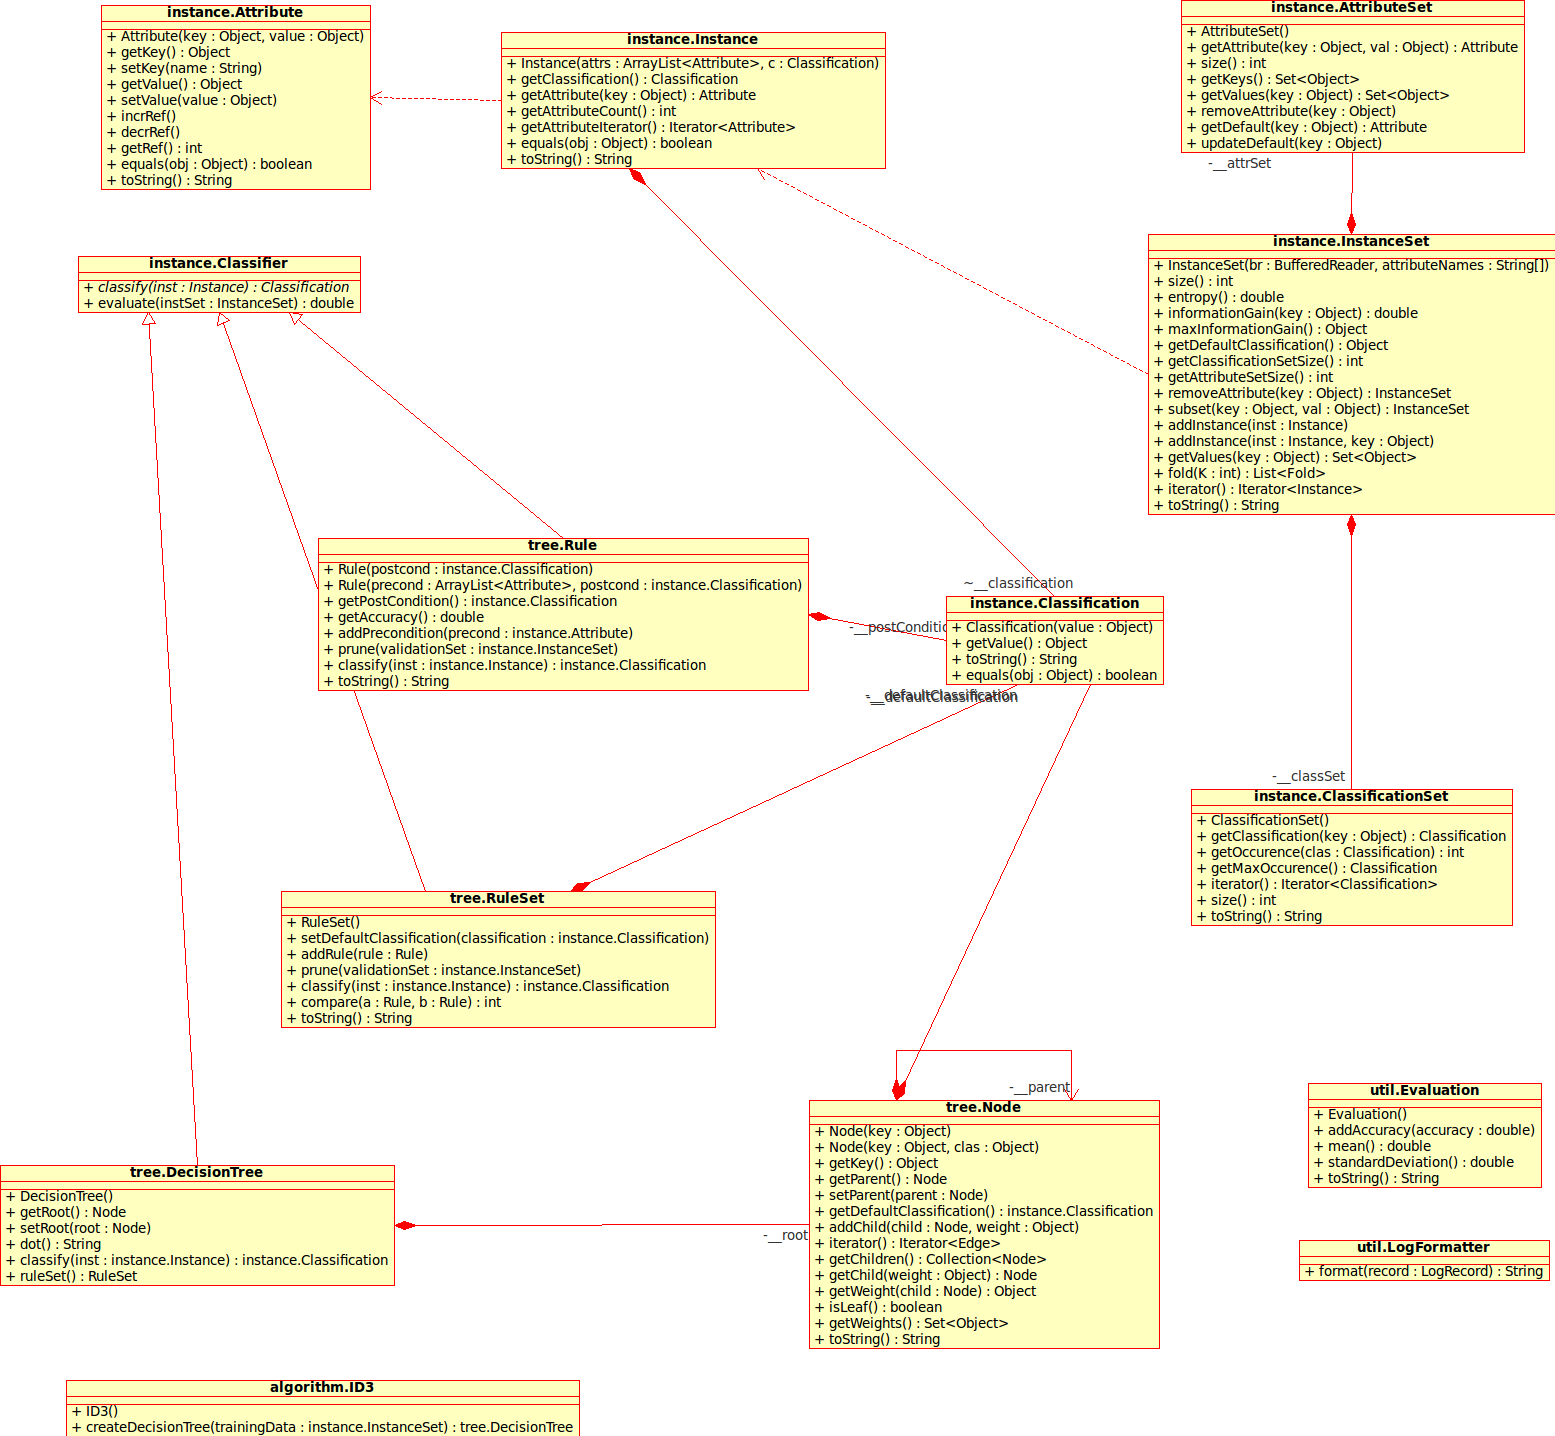
\includegraphics[angle=90,width=\textwidth,height=!]{uml}
  \end{center}
  \caption{UML class diagram}
  \label{fig:uml}
\end{figure} 


%----------------------------------------
% Bibliography
%----------------------------------------
\bibliography{bibliography}
\bibliographystyle{plain}


%--------------------------------------------------
\end{document}
